%% LaTeX2e class for student theses
%% sections/preliminary.tex
%% 
%% Karlsruhe Institute of Technology
%% Institute for Program Structures and Data Organization
%% Chair for Software Design and Quality (SDQ)
%%
%% Dr.-Ing. Erik Burger
%% burger@kit.edu
%%
%% Version 1.1, 2014-11-21


\chapter{Preliminary Definitions}
\label{ch:Preliminary}

In the following chapter we want to define and terms, models and logic used throughout this thesis. We skip the explanation of first-order logic, which we presume to be known by the reader.

\section{Introducing Cyber-Physical-Systems}
\label{sec:pre:cps}

In this thesis we take a close look at \textbf{CPS}. These are systems in which a physical aspect or value is controlled by a computer (program). For example, an aircraft control system in which the computer exerts a form of speed control on the airplane would be a CPS. 

For our purposes we also refer to CPS as \textit{Hybrid Systems}, in which discrete values (in the control program) and continuous values (in the physical world) coexist. The difficulty in analyzing these kinds of systems stems from the ``hybridness'' of the systems: There is always some form of translation necessary to go from the program (discrete values) to the physical (continous reals) world. 

\subsection{Modelling CPS as Hybrid Automata}

Two different modelling approaches exist for CPS, the first one we now explain are hybrid automata. Formally they are defined to have the following components (From~\cite{Heinzinger2000b}):
\begin{quote}
		\begin{description}
			\item[\textit{Variables}]A finite set \(X = \{x_1,\dots , x_n\}\) of real numbered variables. The number \(n\) is called the dimension of \(H\). [...]
			\item[\textit{Control graph}]A finite directed multigraph \((V, E)\). The vertices in \(V\) are called control modes. The edges in \(E\) are called control switches.
			\item[\textit{Initial, invariant, and flow conditions.}]Three vertex labeling functions \(init\), \(inv\) and \(flow\) that assign to each control mode \(v\in V\) three predicates. [...]
			\item[\textit{Jump conditions}]An Edge labeling function jump that assigns to each control switch  \(e \in E\) a predicate.
			\item[\textit{Events}]A finite set \(\Sigma\) of events, and an edge labeling function event: \(E \rightarrow \Sigma\) that assigns to each control switch an event.
		\end{description}
\end{quote} 

Based on non-deterministic finite automata (NFA), they are easy to understand for humans and serve well to model the abstract behavior of hybrid systems. A possible hybrid automatacan be seen in Fig.~\ref{fig:automata}. It describes the behavior of a controller controlling the train on a rail section. A train is therefore always either traveling freely (accelerating)  or being slowed. The biggest difference to NFAs is apparent when looking inside both states: They are continuous, so there is no single value assigned to the train's acceleration but rather a description of the behavior of the value over time is given. This means, that the single state "accelerate" can also be seen as a continous flowing assignment of values according to the specified differential equation.~\cite{platzer2010b}.

The system still obviously exhibits its continuous behavior, as any change to the acceleration also brings the change of speed and location. As the train comes passes arbitrarily chosen point \emph{SB}, the controller automatically assigns a discrete negative value to the train's acceleration, decelerating it, so it slows down. In the brake state the train again follows the equations of linear motion with continuous assignment, only that the guard \(v \geq 0\) makes sure the train never travels backwards (with a negative velocity), but rather at some point starts accelerating again according to the discrete assignment in the state change between brake and accelerate.

\begin{figure}[ht!]
	\centering
	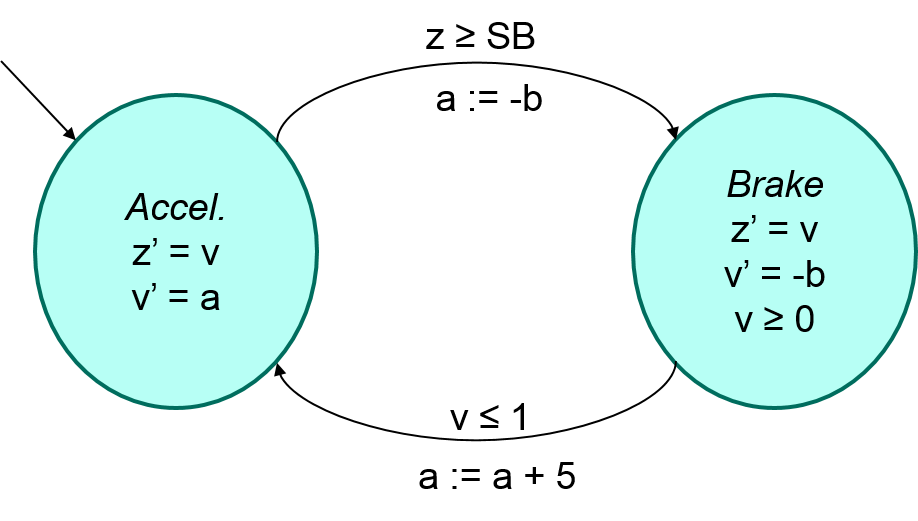
\includegraphics[width=1.0\textwidth]{images/automata}
	\caption{A simple Hybrid Automata~\cite{platze2010b}.}
	\label{fig:automata}
\end{figure}

\subsection{Modelling CPS as Hybrid Programs}

As we are using \keym~for verification, which uses Hybrid Programs (HP), we also have to introduce the syntax of hybrid programs. They follow the syntax depicted in table~\ref{tab:hp}, whereby \(\theta_i\) are terms, \(x_i \in \Sigma\) are state variables and \(\chi\) is a formula of first-order logic~\cite{platzer2010b}.

As an example we take a look at the hybrid program notation of a train control sustem (See Fig.~\ref{fig:etcs_hp}). As can be seen, the state variable \(x\) is first assigned the state accelerate, this corresponds to the hybrid automaton's (See Fig.~\ref{fig:automata}) starting state of the system. In line 3 we can see the hybrid program syntax being an extension of first-order logic: Only if \(q=accel\) \textbf{and} \(z \geq SB\) are true can this case be enacted (corresponding to the state change from accel. to brake in the automaton).

\begin{table}
	\begin{tabular}{p{5cm} | p{4cm} | p{6cm} }
		notation & statement & effect \\ \hline
		\(x := \theta\) & discrete assignment & assigns term \(\theta\) to variable \(x\) \(\in\) \(V\) \\
		\(x := \ast\) & nondet. assignment & assigns any real value to \(x \in V\) \\
		\(x^{\prime}_1 = \theta_1 \wedge ... \newline
		... \wedge x^{\prime}_n = \theta_n \wedge \chi\) & continuous evolution & diff. equations for \(x_i \in V\) and terms \(\theta_i\),\newline
		with formula \(\chi\) as evolution domain \\
		\(?\chi\) & state check & test formula \(\chi\) at current state \\
		\(\alpha;\beta\) & seq. composition & HP \(\beta\) starts after HP \(\alpha\) finishes \\
		\(\alpha \cup \beta\) & nondet. choice & choice between alternatives HP \(\alpha\) or \(\beta\) \\
		\(\alpha^\ast\) & nondet. repetition & repeats HP \(\alpha\) \(n\)-times for any \(n \in \mathbb{N}\) \\
		%\it{do} \(\alpha\) \it{until} \(\chi\) & evolve until &  evolve HP \(\alpha\) until \(\chi\) holds \\
	\end{tabular}
	\caption{Syntax of Hybrid Programs (HP)~\cite{platzer2010b}.}
	\label{tab:hp}
\end{table}

\begin{figure}[ht!]
	\(q := accel;\)\newline
	\(((?q = accel; z^{\prime}= v, v^{\prime}= a)\) \newline
	\(\cup~(?q = accel \wedge z \geq SB; a := -b, q:= brake; ?v \geq 0)\) \newline
	\(\cup~(?q = brake; z^{\prime}=v, v^{\prime}= -b \wedge v \geq 0)\) \newline
	\(\cup~(?q = brake \wedge v \leq 1; a := a+5; q := accel))^\ast\)
	\caption{A simplified train control system as a Hybrid Program~\cite{platzer2010b}.}
	\label{fig:etcs_hp}
\end{figure}

\section{Dynamic Logic}
\label{sec:pre:DL}

Dynamic logic is a multi-modal logic and has two basic operators (one of which is relevant to this thesis): Either \textit{safety} (\([]\)) in which a first-order-logic formula \(\phi\) holds true in all exit states of the program \(\alpha\). Or \textit{liveness} (\(\langle\rangle\)), where a possible execution of the program \(\alpha\) exists, after which the first-order-logic formula \(\phi\) holds. In this paper only the safety operator is used. They can be expressed as in Eq.~\ref{eq:ddl}, whereby \(\alpha\) denotes the (hybrid) program that is enacted, and \(\phi\) is the postcondition expressed in first-order-logic.

\begin{equation}
	\begin{split}
		Safety: [\alpha]\phi \\
		Liveliness: \langle\alpha\rangle\phi \equiv \neg ([\alpha] \neg \phi) \\
	\end{split}
	\label{eq:ddl}
\end{equation}

\subsection{Differential Dynamic Logic}
\label{subsec:DDL}

While dynamic logic in itself was not specifically devised for hybrid programs, this means we need a way to express differential equations, as most continuous movement or behavior is expressed by differential equations. DDL or d\(\mathcal{L}\), the language also used by our verification tool \keym, has ways to express differential equations as can be seen in Table~\ref{tab:hp}.

\subsection{JML: Verification of Java Programs using \key}
\label{subsec:jml}

In this thesis we also deal with the verification of Java programs (the control programs of our cps). We now want to introduce the Java Modelling Language \textit{JML}, which is used to model specification of Java classes/modules or single methods. JML is based on the Design-By-Contract premise, which means that the user and the Java classes have a contract with each other which defines the input and output conditions of the program~\cite{keybook2007}. JML is then listed as a comment in the Java sourcecode right before the method in question~\cite{fmcoKeYTutorial06}. For example the JML code for a method in question could look like this:


\definecolor{darkgreen}{rgb}{0.0, 0.2, 0.13}
\lstset{language=Java,captionpos=b,tabsize=3,frame=lines,keywordstyle=\color{blue},commentstyle=\color{darkgreen},stringstyle=\color{red},numbers=left,numberstyle=\tiny,numbersep=5pt,breaklines=true,showstringspaces=false,basicstyle=\footnotesize,emph={label}}
\begin{lstlisting}[label=lst:jml_example]

/*@ public normal_behavior
   @ requires a >= 0
   @ ensures b >= 2
  */
  public int getPlusTwo(int a) {
  	b = a + 2;
  	return b;
}

\end{lstlisting}

As one can see, the JML proof obligation needs to have the access level and a name and (for our purposes) always will have a \textit{requires} precondition that must hold true before the method is called for all arguments or some class variables and a \textit{ensures} postcondition clause, that has to hold true for all exit states of the method (where the precondition was true before calling it). This means the JML above could also be expressed in Java Dynamic Logic as:

\begin{equation}
	a \geq 0 \implies [b := getPlusTwo(a) ] b \geq 2
	\label{eq:jmlddl}
\end{equation}

\section{\keym~as our Verification Tool for Hybrid Programs}
\label{sec:pre:key}

As \key~can only deal with Java programs, but we deal with problems with hybrid systems, we use \keym~as our tool of choice to verify our hybrid models. It is based on \key's source and developed by Andr\'e Platzer at Carnegie Mellon University~\cite{keymaera}. As its backend arithmetic solver we used Wolfram Mathematica~\cite{mathematica}, but \keym~supports other computer algebra solvers as well.

Hybrid Programs are expressed as \textit{regular programs}, but as for example \(\cup\) is not a symbol used in ASCII text, the program notation in the \textit{.key} \keym-files is different (e.g. \(\cup\) as \(++\)), but we will present every hybrid program in the syntax presented above as well as to avoid confusion and adding another layer of abstraction.
